%%%% ijcai09.tex

\typeout{IJCAI-09 Instructions for Authors}

\documentclass{article}
% The file ijcai09.sty is the style file for IJCAI-09 (same as ijcai07.sty).
\usepackage{ijcai09}
\usepackage{graphicx}
%\usepackage{subfigure}
\usepackage[small]{subfigure}
\graphicspath{{.}{ResultWith0.5/}{ColorOrdering/}{othertechniqueresult/1/} {othertechniqueresult/2/} 
{othertechniqueresult/3/} {othertechniqueresult/4/} {othertechniqueresult/5/} {othertechniqueresult/6/}
{othertechniqueresult/7/} {othertechniqueresult/8/}}

% Use the postscript times font!
\usepackage{times}

\usepackage{multirow}

% the following package is optional:
\usepackage{latexsym} 

\title{Perceptually Enhanced Color-to-Gray with Versatile Color-Reordering}
%Perceptually  Enhanced Non-linear Color-to-Gray}
\author{Taekyu Shin\\
Department of Computer Science\\
UMBC \\
shin7@umbc.edu}

\begin{document}

\maketitle

\begin{abstract}
  {\it Perceptually Enhanced Color-to-Gray with Versatile Color-Reordering} will present color-to-gray conversion algorithm which ensures discriminability between different colors based on perceptual intensity of each color. It also allows users to do color-reordering in such a way that it does not compromise perceptual greyscale ordering.This technique incorporates Helmholtz-Kohlrausch predictor to first globally map the colors. Since overly local mapping might distort grey values of constant color regions, we find the general representation of local color differences and use the data to modify the global mapping. Its goal is to successfully find a mapping without compromising color-ordering and distorting greyscale values from constant or neighboring colors.
\end{abstract}

\section{Introduction}

{\it Perceptually Enhanced Non-linear Color-to-Gray}
Color-to-gray conversion is useful in many image processing applications and media today. Unfortunately, converting the intensity component of colors to greyscale values may not not result in ideal color conversion for some purposes. The color-conversion method should achieve a few important aspects to ensure the appropriate containment of original color information. First of all, color discriminality is sometimes compromised through color-to-grey conversion because the mapping of different color values to the same greyscale would result in loss of the image features. Previous research has shown that such feature discriminality is very achievable for various images, using global and local mapping. Local mapping methods can achieve color or feature discriminality since it is easier to aim at differentiating grey values from different colors, yet inhomogeneously convert color values to grey ones globally. On the other hands, global mapping can easily accomplish appropriate color-ordering and homogeneous color conversion, but it may be difficult to preserve feature characteristics of images, sometimes cause artifacts. Previously, many papers have presented using either or both the mappings, accomplishing such aspects in most cases. However, it is obviously challenging to work for all cases because some aspects may co-offset each other. Specifically, overemphasizing color differences for feature discriminability globally may bring about inaccurate color-ordering. Local statistical tweaking to avoid inaccurate color-ordering may result in failure of mapping consistency or visually unnatural mapping. \\
 The goal of this paper is to create perceptually accurate color-to-gray conversion enhanced with feature discriminality, removing distortion of greyvalues from the constant colors and many different aspects in accordance with \cite{cadik08perceptual}, which shows that grey images with perceptual accuracy result in visually pleasing scenes through a user-subjective study that involves a decent number of participants. \\
 In this paper, we use a global mapping and a local mapping. Our global mapping incorporates Helmholtz Kohlrausch(H-K) predictor to achieve perceptually accurate images. \cite{Nayatani97}  Although we use a local mapping, the local mappings work in a similar way to global mapping since both methods combined can achieve many good aspects of each global and local mapping at the same time, and our experiment shows that it achieved good aspects of each without adverse traits. For example, although it considers local color differences, it does not cause artifacts.(See Figure ~\ref{fig:artifactex}) \\
 Although with decent qualities such as consistent mapping and discriminability of greyscale,  we believe that there are still needs for improvements over satisfying color-ordering results. In \cite{kim09_c2g}, it is also indicated that inverse color-ordering depending on saturation may come useful. Our technique demonstrates grey-scale re-ordering with user-defined variable. It allows end-users to manipulate color-reordering depending on the hue and saturation. Since the H-K predictor in this technique might not be able to incorporate high dynamic range of colors properly. We also use an algorithm that deals with high dynamic range, which is similar to that of \cite{journals/pr/GrundlandD07}. As a result, out experiments display decent quality of color conversion and at the same time, user-controllable color-reordering results without any noticeable artifacts. In other words, this perceptual method may prevent over-exaggeration of dynamic range colors, properly dealing with it and display psychologically decent results of color-orderings to its viewers. \\
 All in all, this visually accurate mapping technique can bring viewers right information of what original colors may be. Also it gives them freedom to adjust the intensity ordering in perceptually decent ways. We also explored using the Hunt color model \cite{Hunt} and CIECAM02 color model. However, we concluded that it may not be suitable since it does not strongly consider variance over saturation shift, which does not fit the aim of our technique, whose case is similar to \cite{Smith_apparentgreyscale}. Also, it may be far too heavy algorithm to use since it is required to be interactive with users. Additionally, we avoided using CIELab color space for the global mapping because it may not allow as an accurate mapping since it is based on the wrong Von Kries model and nor it neglects many perceptive affects depending on surroundings.\cite{Fairchild2004_1}


\begin{figure}[h]
  \begin{center}
    \subfigure[Input Image]{\label{fig:edge-a}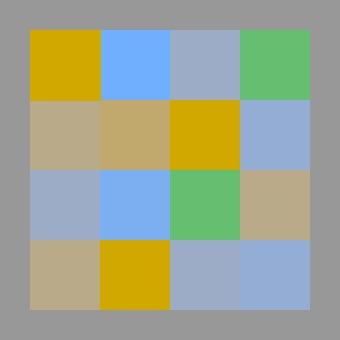
\includegraphics[width=1.1in]{input4x4.jpg}}
    \subfigure[Smith et. al]{\label{fig:edge-b}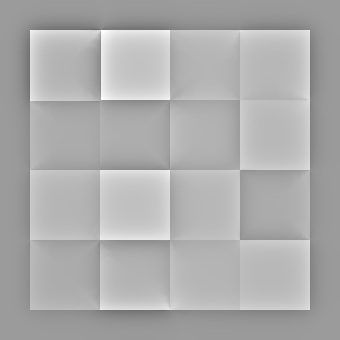
\includegraphics[width=1.1in]{smithartifact.jpg}}
    \subfigure[Our Result]{\label{fig:edge-c}
\includegraphics[width=1.1in]{mymethod4x4.jpg}}\\

    \subfigure[Input Image]{\label{fig:edge-d}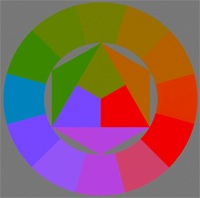
\includegraphics[width=1.1in]{hueorder.jpg}}
    \subfigure[Gooch et. al]{\label{fig:edge-e}
\includegraphics[width=1.1in]{goochartifact.jpg}}
    \subfigure[Out Result]{\label{fig:edge-f}
\includegraphics[width=1.1in]{mymethodhueorder.jpg}}

  \end{center}
  \caption{Notice that Smith et. al and Gooch et. al possibly can cause artifacts since they use local mappings. However, our local
mapping can successfully generate images since we apply it globally and also achieve decent color ordering (See \ref{fig:edge-f})}
  \label{fig:artifactex}
\end{figure}



\section{Related Work}
Previously, \cite{BalaEschbach} presented a space-dependant technique where luminance variance occurs when it contains high frequencies by adding filtered chroma channel to the luminance channel. To avoid over-emphasizing the values in bright areas in original images, local adjustment takes place and its sign is taken from the lightness channel. \\\\
\cite{journals/pr/GrundlandD07} presents a method where it converts RGB to YPQ color space and using its own pca technique, it achieves visually pleasing color discriminability. However, it sometimes brings about over-exaggeration in images with wide gamuts due to inaccuracy of perceptual differences between the two color space pixel differences. \\\\
\cite{cadik07color_to_gray}  proposed a technique that uses an image’s gradient field by colour differences in the Coloroid color space, which is a useful tool to represent aesthetical relationships between colors. The method has a linear complexity and thus, it can convert images with high resolutions, and perceptually pleasing. Related to this paper, \cite{cadik07color_to_gray}  maps less saturated colors to brighter greyscale values. \cite{kim09_c2g} \\\\
One of the most contemporaneous research \cite{Gooch05color2gray:salience-preserving} considers pixel chromatic difference from neighboring pixels. This Color-to-gray conversion algorithm is based on the human visual system sensitive to local changes. Using 3 user-defined variables, it successfully accomplishes the general color-to-gray problems. However, its complexity is high. The worst case is O($N^4$), the ideal case with some specific parameter is O($N^2$). Related to this paper, this research introduces user-defined color-ordering, which is versatile, although color discriminability may not be ideal in some cases. \\\\
Re-coloring Images for Gamuts of Lower Dimensions \cite{Rasche05re-coloringimages} proposes a linear transform that maps the greyscale to the color difference using an error function. The linear color mapping onto the axis is optimized for color differences. The quantized color present should have an impact on the results Therefore, the speed is subject to gamut ranges, which may cause heavy computation. One of the techniques that are globally consistent, but prone to quantization artifacts due to constrained multidimensional scaling. \cite{cadik08perceptual}\\\\
\cite{cadik07color_to_gray} explores Image’s gradient field by colour differences in the Coloroid color space, which is a useful tool to represent aesthetical relationships between colors. Then, based on orthogonal projection, it corrects inconsistent gradients. The gradient formula based on color order system defined by Coloroid color space allows different discriminability of different colors. \\\\
\cite{Smith_apparentgreyscale} explores using Nayatani color model to achieve perceptually sensible technique. Using the perceptual color mode, it achieves visually pleasing results. The Nayatani color model resolves many negative effects just like the hunt color model although not as comprehensive. As a result, it accomplishes a visually pleasing conversion. It also decomposes an image into many Laplacian pyramid levels to visually and artificially discriminate the local color differences. However, because of the local mapping with an exponent power function, it sometimes causes unexpected gradient-like artifacts. As a result, it does not do visually homogeneous mappings among neighboring pixels due to the dynamic local mapping not considering mapping consistencies.\\\\




\section{Design Goals}
\textbf{Preserving Saturation and Hue Contrasts:} Colors that are visually distant to each other should be mapped to different values of greyscale. Our post-processed mapping well achieves this.\\
\textbf{Preserving Luminance Consistency:} Through luminance and chrominance variance, arbitrary colors should not fall into the same greyscale color. For example, dark red neon signs of stores should not have the same color as bright blue sea. These effects can be naturally dealt with by using the perceptual techniques used in our method. However, it may not be accomplished when users set the parameter to not 1.\\
\textbf{Robust Color Ordering:} Depending on hue and saturation components, the result greyscale should be distinguishable. For instance, image areas that have hue gradients with the same color should have different greyscale colors.(See Figure \ref{fig:ColorOrderings}) Also, it should be the case of the same hue with different saturation as well. Additionally, in the former or latter case, the greyscale ordering should be preserved after conversions. In our method, the same hue with saturation gradients may not be preserved since it is one of the goals of our designs.\\
\textbf{Mapping Accuracy:} After the color-to-grey conversion, viewers should feel the same amount of intensity from each areas and colors.\\
\textbf{Perceptually Pleasing Greyscale:} Based on Cadik's result, we believe that achieving mapping accuracy also meets this goal.\\\
\textbf{Global Mapping Consistency:} The same colors in any areas of an image should have the same greyscale. To be specific, the same reddish color on the left and right side of the image should look the same after conversions.\\
\textbf{Algorithm Complexity:} Since this technique requires a user input, it should be fast enough for users to be able to interact. In other words, users should be able to watch greyscale changes depending on their user input so that they can adjust to get what they intend to gain.(Please see Figure ~\ref{fig:ColorOrderings})\\


\begin{figure}[t]
  \begin{center}
    \subfigure[Input Image]{\label{fig:edge-a}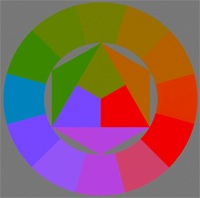
\includegraphics[width=0.8in]{hue-order.jpg}}
    \subfigure[(p=1)]{\label{fig:edge-b}
\includegraphics[width=0.8in]{hue-order-p=1.jpg}}
    \subfigure[(p=0)]{\label{fig:edge-c}
\includegraphics[width=0.8in]{hue-order-p=0.jpg}}
    \subfigure[(p=-1)]{\label{fig:edge-d}
\includegraphics[width=0.8in]{hue-order-p=-1.jpg}} \\

    \subfigure[Input Image]{\label{fig:edge-a}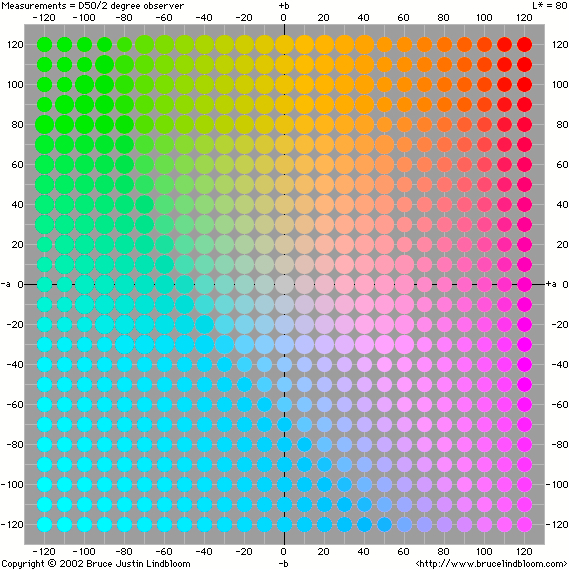
\includegraphics[width=0.8in]{hue-order2.jpg}}
    \subfigure[(p=1)]{\label{fig:edge-b}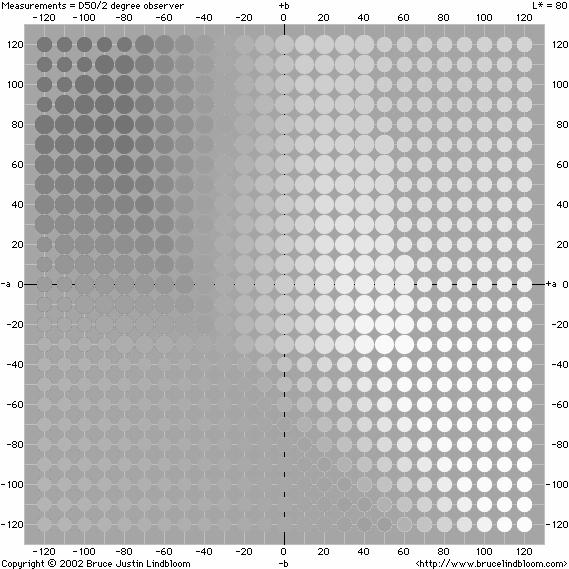
\includegraphics[width=0.8in]{hue-order2-p=1.jpg}}
    \subfigure[(p=0)]{\label{fig:edge-c}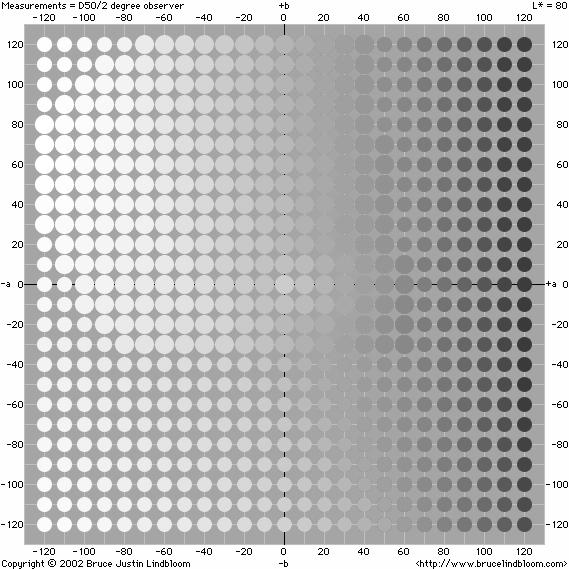
\includegraphics[width=0.8in]{hue-order2-p=0.jpg}}
    \subfigure[(p=-1)]{\label{fig:edge-d}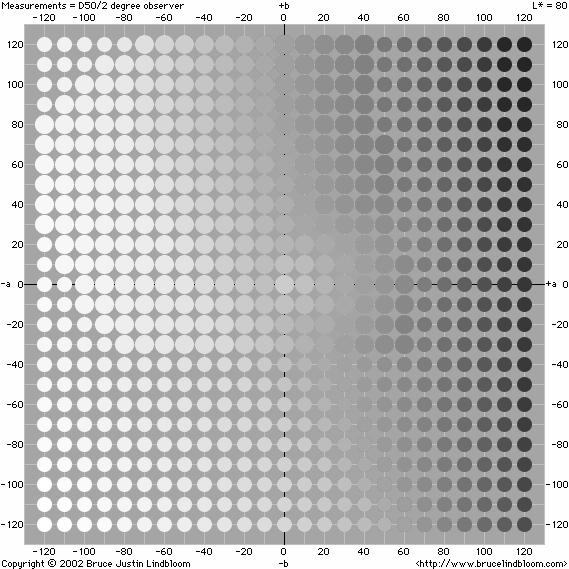
\includegraphics[width=0.8in]{hue-order2-p=-1.jpg}} \\

    \subfigure[Input Image]{\label{fig:edge-a}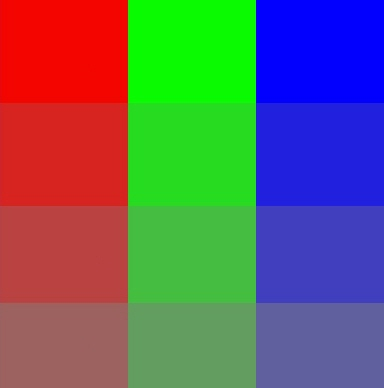
\includegraphics[width=0.8in]{saturation.jpg}}
    \subfigure[(p=1)]{\label{fig:edge-b}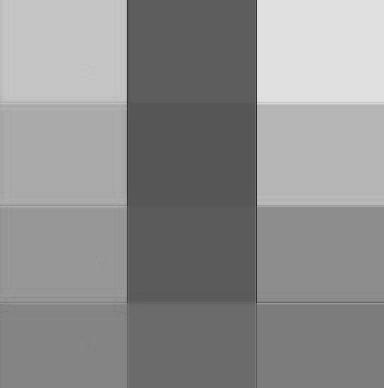
\includegraphics[width=0.8in]{saturation-p=1.jpg}}
    \subfigure[(p=0)]{\label{fig:edge-c}
\includegraphics[width=0.8in]{saturation-p=0.jpg}}
    \subfigure[(p=-1)]{\label{fig:edge-d}
\includegraphics[width=0.8in]{saturation-p=-1.jpg}} 

  \end{center}
  \caption{The result varies depending on user variables. Users can manipulate the hue ordering and saturation ordering as well. Please notice that the input image (a), (c) represent colors with different hue angles. The input image (i) has the same hue in each column. Depending on the rows, only saturation varies. Users may choose p=-1 to get a more dramatic and extreme result.}
  \label{fig:ColorOrderings}
\end{figure}


\section{Algorithms}
\textbf{Overall Steps} \\
1. Global Modification: Use Helmholtz-Kohlrausch(H-K) predictor to globally map colors to greyscale. \\
2.1 Do CIELab color space conversion and YPQ color space conversion.\\
2.2 Get local pixel differences using Gaussian distributed neighborhood pixels.\\
2.3 Using the color differences, define a Component Axis similar to Primary Component Analysis. \\
2.4 Project each pixel value using the axis to get color differences.\\
2.5 Apply the values to the intensity values extracted from H-K predictor.

\subsection{Global Luminance Mapping}
In \cite{cadik08perceptual}, it is stated that visually accurate results also demonstrate visually pleasing image conversions in general. Therefore, our global mapping focuses on perceptually accurate mapping. Since one of the primary traits in this paper is to differ difference in hues and saturations, we disregard complex models such as the Hunt, CIECAM02 model because they do not consider H-K effects, and H-K predictors fit our design goals.(saturation-hue discriminability) . To do that, we incorporate Nayatani's estimation method for H-K effect. \cite{Nayatani98} Because our algorithm is designed to deal with high dynamic range values, we decided to choose $L_{VAC}$ over $L_{VCC}$.(\cite{Smith_apparentgreyscale} observes $N_{VCC}$ may map quite a range or colors to high-dynamic ranges.) However, the result of this mapping is somehow problematic. It does not lead to distinguishable greyscales from different hues. We resolve it by applying another mapping.(See Figure \ref{fig:nayatani})

\begin{figure}[h]
  \begin{center}
    \subfigure[Input Image]{\label{fig:edge-a}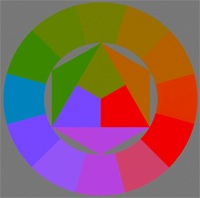
\includegraphics[width=1.5in]{hueorder.jpg}}
    \subfigure[Our Global Mapping]{\label{fig:edge-b}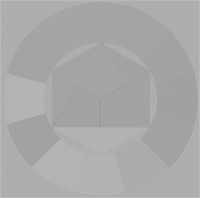
\includegraphics[width=1.5in]{colororder2_Nayatani.png}}
  \end{center}
  \caption{The result of Nayatani's $L_{VAC}$ method. The greyscale between different hues is not noticeable.}
  \label{fig:nayatani}
\end{figure}

\begin{figure}[h]
\centering
 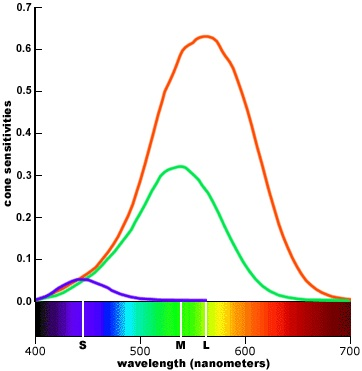
\includegraphics[width=1.5in]{rodconecolors.jpg}
\caption{Due to distribution and amount of cons and rods, our human visual systems respond more to certain colors such as red. [Glassner et al 1995]}.

\label{fig:rodconeresponses}
\end{figure}

\subsection{Local Difference Analysis and Color-Reordering}
 We resolve hue discriminability by incorporating the rod-cone response theory.  Also, a method to manipulate color-ordering is in this post-processing. Our human vision system recognizes more of certain colors. For example, Figure 2 suggests that red can be more dominating than colors such as blue. Since CIELab space\footnote{It may also be applicable to use YPQ color space instead of CIELab space. For YPQ space conversion, see Appendix B.} reflects on the perceptual aspects, we use local color differences between RGB space and CIELab space, which is similar to \cite{journals/pr/GrundlandD07}. The use of Local color differences similar to that of \cite{Gooch05color2gray:salience-preserving}. However, since \cite{Gooch05color2gray:salience-preserving} has $N^4$ complexity in worst case. To make it faster, by using gaussian distributed random variables, we pick a random neighborhood pixel to calculate the color difference. We define R, G, B as the R,G,B component of each pixel:

\begin{eqnarray}
\Delta R_i=R_i-R_{neighbor} \\
\Delta G_i=G_i-G_{neighbor} \\
\Delta B_i=B_i-B_{neighbor}
\end{eqnarray}
\begin{eqnarray}
\Delta D_i = \sqrt{ \Delta R_i^2 + \Delta G_i^2 + \Delta B_i^2 }
\end{eqnarray}

We also define :
\begin{eqnarray}
\Delta L_i=L_i-L{neighbor} \\
\Delta a_i=a_i-a_{neighbor} \\
\Delta b_i=b_i-b_{neighbor}
\end{eqnarray}

After normalization of $\Delta L$, we get the difference between the human visual response and each RGB components. which we use later to exaggerate hue differences in greyscale. Also, to be able to manipulate color-ordering with user-defined variable, we place the user-defined variable p in the below equation. $sign$ is a function that gets the sign of the parameter value.

\begin{eqnarray}
c_i = \frac { \Delta D - \frac{\Delta L}{ C }  } {\Delta D } \\
\Delta D_2 = \Delta L^3 + \Delta a^3 + \Delta b^3 \\
sign_i = sign(  \Delta D * (1-p) + \Delta D_2 * p ) \\
axis_a = \Sigma_i^n sign_i * c_i * a_i  \\
axis_b = \Sigma_i^n sign_i * c_i * b_i 
\end{eqnarray}

$C$ is an experimental constant. We use $C$ to normalize L values properly to fit $\Delta D$. According to CIELab ranges, we should put a value between [1, 1.1]. Through our experiments, we define C as 0.67. For the $sign$ function, we use both sign functions defined in \cite {cadik07color_to_gray} and also by \cite{journals/pr/GrundlandD07}. We define an axis to do IADCA(Image Adaptive Component Analysis), which is similar to Predominant Component Analysis of \cite{journals/pr/GrundlandD07}, which is also adapted from PCA(Principal Component Analysis). The reason we chose IADCA is that according to \cite{Hunt}, how we perceive a color is related to surrounding gamuts. It implies to us that depending on gamut ranges, the same color can be perceived to be a little bit brighter or darker. (See Figure \ref{fig:humanvisionsystem}) By adapting color difference and finding a representitive axis of the difference, we can do a vivid conversion that saves the perceived colors. This is why we defined the axis adaptive to the input image.

\begin{figure}[h]
  \begin{center}
    \subfigure[Input Image]{\label{fig:edge-a}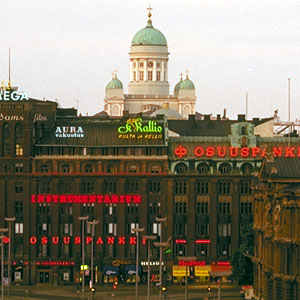
\includegraphics[width=1.1in]{pascu.jpg}}
    \subfigure[CIELab]{\label{fig:edge-b}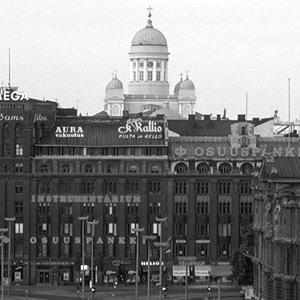
\includegraphics[width=1.1in]{pascugrey.jpg}}
    \subfigure[Our Result]{\label{fig:edge-b}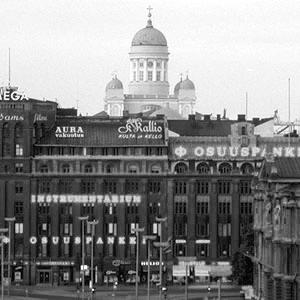
\includegraphics[width=1.1in]{pascu_ourresult.jpg}}
  \end{center}
  \caption{How human vision system works. Notice that the red sign is obvious when looking at the colored picture. The white sign is not obvious relatively. After the conversion, the red sign is no longer as obvious, and the white sign becomes obvious.}
  \label{fig:humanvisionsystem}
\end{figure}


\subsection{Modification of Greyscale with Gradient Component Analysis}
 After the global mapping, the primary goal of this post-processing is to accomplish decent color-discriminability and color-reordering. This post-processing gives freedom to manipulate intensity of greyscale and ordering. It is perceptually appropriate because the axis reflects on the fact that certain colors have stronger impressions on how human visual system conceives those colors.

\section{Results}
 We implemented our technique in Matlab. We measured the speed with the built-in matlab function 'cputime.' It took 0.3744 seconds on a laptop PC with a i7 CPU 1.76GHz and 4 GB memory for a 200x198x24bit-color image. We did not use gamma correction. We compared our result to those of previous techniques included in \cite{kim09_c2g}, whose results were also taken from \cite{cadik08perceptual}. As you can see from Figure \ref{fig:ColorOrderings}, we successfully generate greyscale whose color-orderings can be manipulated by users. Not only saturation ordering can be manipulated, hue ordering manipulation can be achieved with perceptually decent results. Our result shows decent hue color-reordering compared to previous techniques as well. In terms of feature discriminability, it shows decent feature discriminability because we use an image-dependant axis to project color differences. (Please see Figure \ref{fig:resultcomparison}) In terms of mapping accuracy, our method demonstrates decently accurate mapping in most cases. Our technique achieves area-independant mapping.

\begin{figure*}[t]
  \begin{center}
    \subfigure[Input]{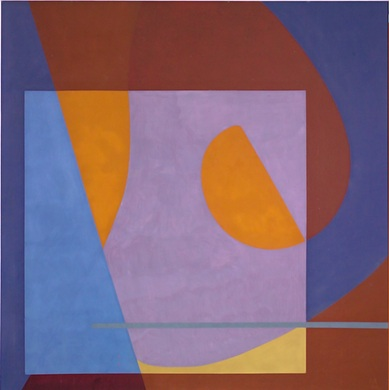
\includegraphics[width=0.6in]{1.jpg}}
    \subfigure[Ours(p=1)]{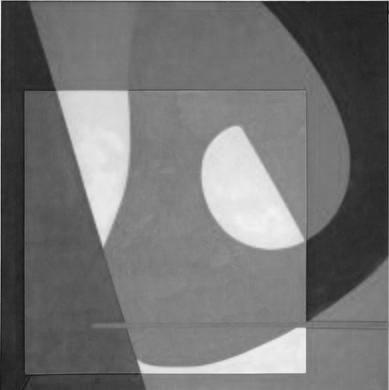
\includegraphics[width=0.6in]{1-mine-p=1.jpg}}
    \subfigure[Ours(p=-1)]{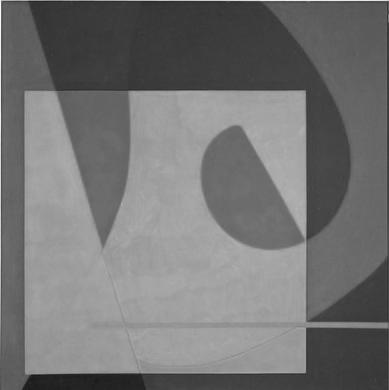
\includegraphics[width=0.6in]{1-mine-p=-1.jpg}}
    \subfigure[CIE Y]{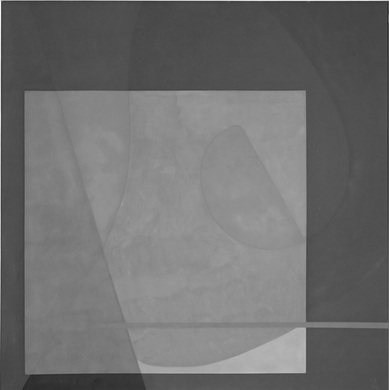
\includegraphics[width=0.6in]{1-y.jpg}}
    \subfigure[Bala]{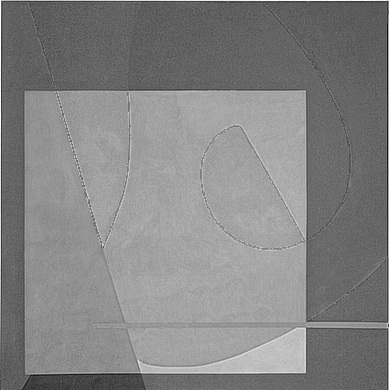
\includegraphics[width=0.6in]{1-bala.jpg}}
    \subfigure[Gooch]{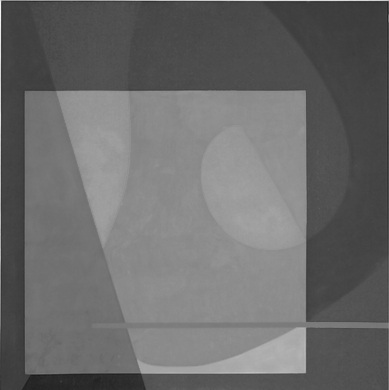
\includegraphics[width=0.6in]{1-gooch.jpg}}
    \subfigure[Grundland]{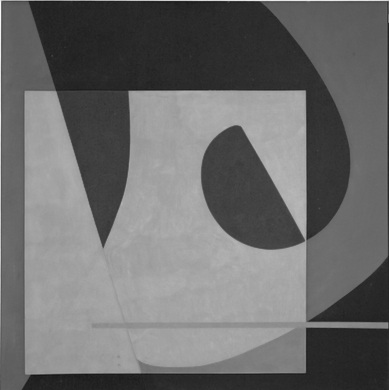
\includegraphics[width=0.6in]{1-grund.jpg}}
    \subfigure[Kim]{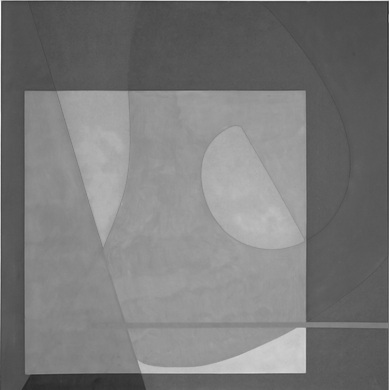
\includegraphics[width=0.6in]{1-kim.jpg}}
    \subfigure[Neumann]{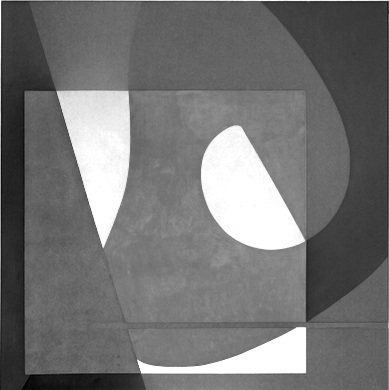
\includegraphics[width=0.6in]{1-neumann.jpg}}
    \subfigure[Rasche]{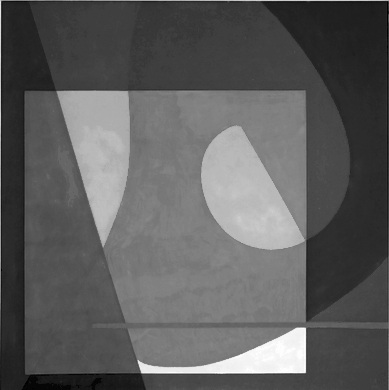
\includegraphics[width=0.6in]{1-rasche.jpg}}
    \subfigure[Smith]{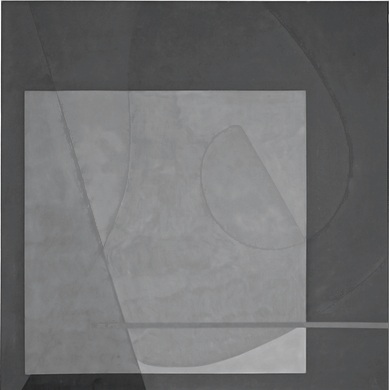
\includegraphics[width=0.6in]{1-smith.jpg}} \\

    \subfigure{
\includegraphics[width=0.6in]{2.jpg}}
    \subfigure{
\includegraphics[width=0.6in]{2-mine-p=1.jpg}}
    \subfigure{
\includegraphics[width=0.6in]{2-mine-p=-1.jpg}}
    \subfigure{
\includegraphics[width=0.6in]{2-y.jpg}}
    \subfigure{
\includegraphics[width=0.6in]{2-bala.jpg}}
    \subfigure{
\includegraphics[width=0.6in]{2-gooch.jpg}}
    \subfigure{
\includegraphics[width=0.6in]{2-grund.jpg}}
    \subfigure{
\includegraphics[width=0.6in]{2-kim.jpg}}
    \subfigure{
\includegraphics[width=0.6in]{2-neumann.jpg}}
    \subfigure{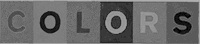
\includegraphics[width=0.6in]{2-rasche.jpg}}
    \subfigure{
\includegraphics[width=0.6in]{2-smith.jpg}} \\

    \subfigure{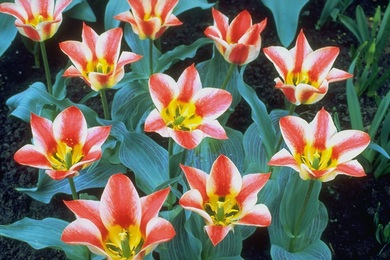
\includegraphics[width=0.6in]{3.jpg}}
    \subfigure{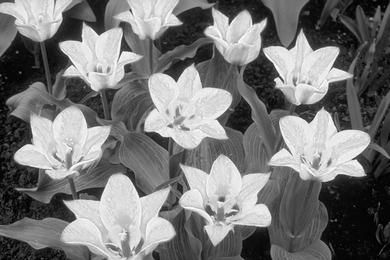
\includegraphics[width=0.6in]{3-mine-p=1.jpg}}
    \subfigure{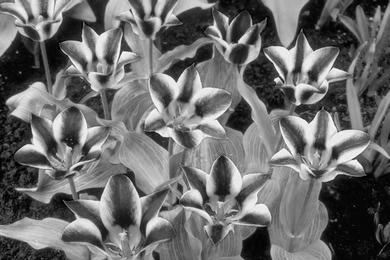
\includegraphics[width=0.6in]{3-mine-p=-1.jpg}}
    \subfigure{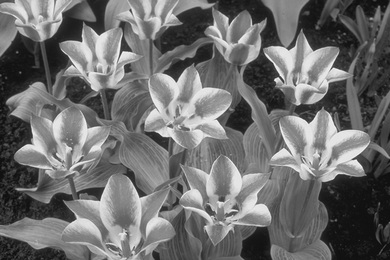
\includegraphics[width=0.6in]{3-y.jpg}}
    \subfigure{\includegraphics[width=0.6in]{3-bala.jpg}}
    \subfigure{\includegraphics[width=0.6in]{3-gooch.jpg}}
    \subfigure{\includegraphics[width=0.6in]{3-grund.jpg}}
    \subfigure{\includegraphics[width=0.6in]{3-kim.jpg}}
    \subfigure{\includegraphics[width=0.6in]{3-neumann.jpg}}
    \subfigure{\includegraphics[width=0.6in]{3-rasche.jpg}}
    \subfigure{\includegraphics[width=0.6in]{3-smith.jpg}} \\

    \subfigure{\includegraphics[width=0.6in]{4.jpg}}
    \subfigure{\includegraphics[width=0.6in]{4-mine-p=1.jpg}}
    \subfigure{\includegraphics[width=0.6in]{4-mine-p=0.jpg}}
    \subfigure{\includegraphics[width=0.6in]{4-y.jpg}}
    \subfigure{\includegraphics[width=0.6in]{4-bala.jpg}}
    \subfigure{\includegraphics[width=0.6in]{4-gooch.jpg}}
    \subfigure{\includegraphics[width=0.6in]{4-grund.jpg}}
    \subfigure{\includegraphics[width=0.6in]{4-kim.jpg}}
    \subfigure{\includegraphics[width=0.6in]{4-neumann.jpg}}
    \subfigure{\includegraphics[width=0.6in]{4-rasche.jpg}}
    \subfigure{\includegraphics[width=0.6in]{4-smith.jpg}} \\

    \subfigure{\includegraphics[width=0.6in]{5.jpg}}
    \subfigure{\includegraphics[width=0.6in]{5-mine-p=1.jpg}}
    \subfigure{\includegraphics[width=0.6in]{5-mine-p=-1.jpg}}
    \subfigure{\includegraphics[width=0.6in]{5-y.jpg}}
    \subfigure{\includegraphics[width=0.6in]{5-bala.jpg}}
    \subfigure{\includegraphics[width=0.6in]{5-gooch.jpg}}
    \subfigure{\includegraphics[width=0.6in]{5-grund.jpg}}
    \subfigure{\includegraphics[width=0.6in]{5-kim.jpg}}
    \subfigure{\includegraphics[width=0.6in]{5-neumann.jpg}}
    \subfigure{\includegraphics[width=0.6in]{5-rasche.jpg}}
    \subfigure{\includegraphics[width=0.6in]{5-smith.jpg}} \\

    \subfigure{\includegraphics[width=0.6in]{6.jpg}}
    \subfigure{\includegraphics[width=0.6in]{6-mine-p=1.jpg}}
    \subfigure{\includegraphics[width=0.6in]{6-mine-p=-1.jpg}}
    \subfigure{\includegraphics[width=0.6in]{6-y.jpg}}
    \subfigure{\includegraphics[width=0.6in]{6-bala.jpg}}
    \subfigure{\includegraphics[width=0.6in]{6-gooch.jpg}}
    \subfigure{\includegraphics[width=0.6in]{6-grund.jpg}}
    \subfigure{\includegraphics[width=0.6in]{6-kim.jpg}}
    \subfigure{\includegraphics[width=0.6in]{6-neumann.jpg}}
    \subfigure{\includegraphics[width=0.6in]{6-rasche.jpg}}
    \subfigure{\includegraphics[width=0.6in]{6-smith.jpg}} \\

    \subfigure{\includegraphics[width=0.6in]{7.jpg}}
    \subfigure{\includegraphics[width=0.6in]{7-mine-p=1.jpg}}
    \subfigure{\includegraphics[width=0.6in]{7-mine-p=-1.jpg}}
    \subfigure{\includegraphics[width=0.6in]{7-y.jpg}}
    \subfigure{\includegraphics[width=0.6in]{7-bala.jpg}}
    \subfigure{\includegraphics[width=0.6in]{7-gooch.jpg}}
    \subfigure{\includegraphics[width=0.6in]{7-grund.jpg}}
    \subfigure{\includegraphics[width=0.6in]{7-kim.jpg}}
    \subfigure{\includegraphics[width=0.6in]{7-neumann.jpg}}
    \subfigure{\includegraphics[width=0.6in]{7-rasche.jpg}}
    \subfigure{\includegraphics[width=0.6in]{7-smith.jpg}} \\

    \subfigure{\includegraphics[width=0.6in]{8.jpg}}
    \subfigure{\includegraphics[width=0.6in]{8-mine-p=1.jpg}}
    \subfigure{\includegraphics[width=0.6in]{8-mine-p=-1.jpg}}
    \subfigure{\includegraphics[width=0.6in]{8-y.jpg}}
    \subfigure{\includegraphics[width=0.6in]{8-bala.jpg}}
    \subfigure{\includegraphics[width=0.6in]{8-gooch.jpg}}
    \subfigure{\includegraphics[width=0.6in]{8-grund.jpg}}
    \subfigure{\includegraphics[width=0.6in]{8-kim.jpg}}
    \subfigure{\includegraphics[width=0.6in]{8-neumann.jpg}}
    \subfigure{\includegraphics[width=0.6in]{8-rasche.jpg}}
    \subfigure{\includegraphics[width=0.6in]{8-smith.jpg}} \\


  \end{center}
  \caption{These images are courtesy of Cadik. 6 (c) image in the first row, we used the internal amplifier variable 0.3 instead of 0.5 since it might display some over-exaggeration. Also, we use p=0 for 6 (c) in the 4th row.}
  \label{fig:resultcomparison}
\end{figure*}


\section{Conclusions}


Calabria and  Fairchild indicate that image luminance has a stronger affect on human perceived intensity than chrominance channels. so it is possible that our technique inaccurately or adversely convert color images in some artificial ways. Therefore we may be able to improve this technique further by applying the component axis on chrominance channels.
-- Also, Helmoltz =-> Bezold-Brucke effects can be considered to adapt. It defines the relations between brightness and hue. It may achieve visually correct color-to-grey conversion through images of various hues. However, the implementation method was questionable that we ended up not implementing it.

%%\section*{Acknowledgments}

\appendix
\section{Nayatani Lightness Model}
\cite{Nayatani98}
\begin{equation}
L^*_{VAC} = L^* + [-0.1340 q(\theta) + 0.0872 K_{Br}] s_{uv} L^*
\end{equation}
\begin{equation}
L^* = 116(Y / Y_0)^{1/3} - 16
\end{equation}
\begin{equation}
K_Br = 0.2717 \frac{6.469 + 6.362L_a^{0.4495}}{6.469 + L^{0.4495}_a}
\end{equation}
\begin{equation}
s_{uv} = 13 [(u^{'} - u^{'}_c)^2 +(v^{'} - v^{'}_c)^2]^(1/2)
\end{equation}
\begin{equation}
\theta = \arctan{ \frac{  v^{'} - v^{'} }{u^{'} - u^{'}_c } }
\end{equation}
\begin{eqnarray}
q(\theta) = -0.01585 - 0.03017 \cos\theta - 0.04556 \cos2\theta \\ - 0.02667\cos3\theta - 0.00295\cos4\theta\\ + 0.14592\sin\theta + 0.05084\sin2\theta\\ - 0.01900\sin3\theta - 0.00764\sin4\theta
\end{eqnarray}

\section{YPQ Color Space}
\cite{journals/pr/GrundlandD07} 
\begin{equation}
\left| \begin{array}{c} Y \\ P \\ Q \end{array} \right| = 
\left| \begin{array}{ccc}
0.2989 & 0.5870 & 0.1140 \\
0.5000 & 0.5000 & -1.0000\\
1.0000 & -1.0000&  0.0000
\end{array} \right|
\left|\begin{array}{c} R \\ G \\ B \end{array} \right|
\end{equation}



%% The file named.bst is a bibliography style file for BibTeX 0.99c
\bibliographystyle{named}
\bibliography{ijcai09}


\end{document}

